%\begin{figure}[H]
%	\begin{center}
%		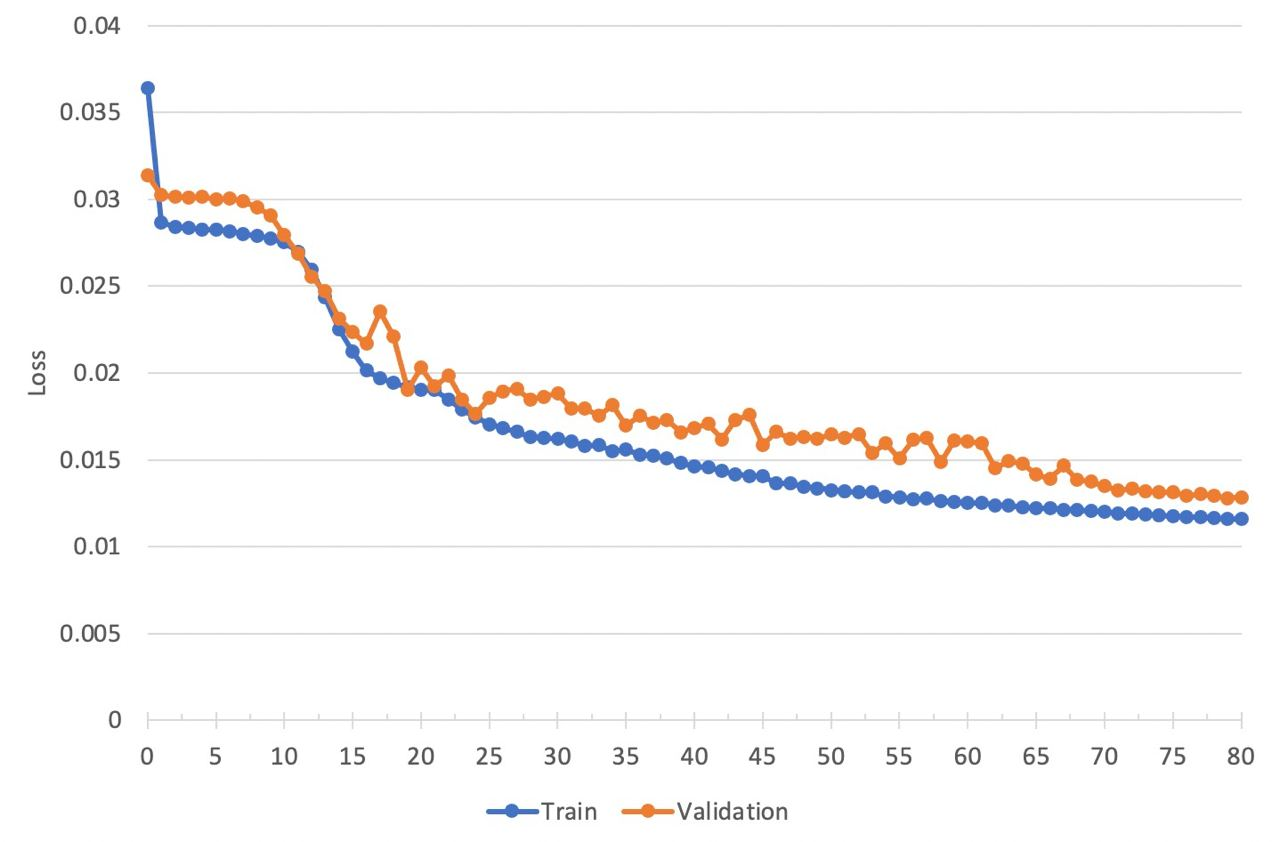
\includegraphics[width=0.5\linewidth]{bilder/nuclei/no-wi.jpg}
%		\caption{Default weight initialization is not suitable}\label{fig:no-wi}
%	\end{center}
%\end{figure}

%\begin{figure}[H]
%	\begin{center}
%		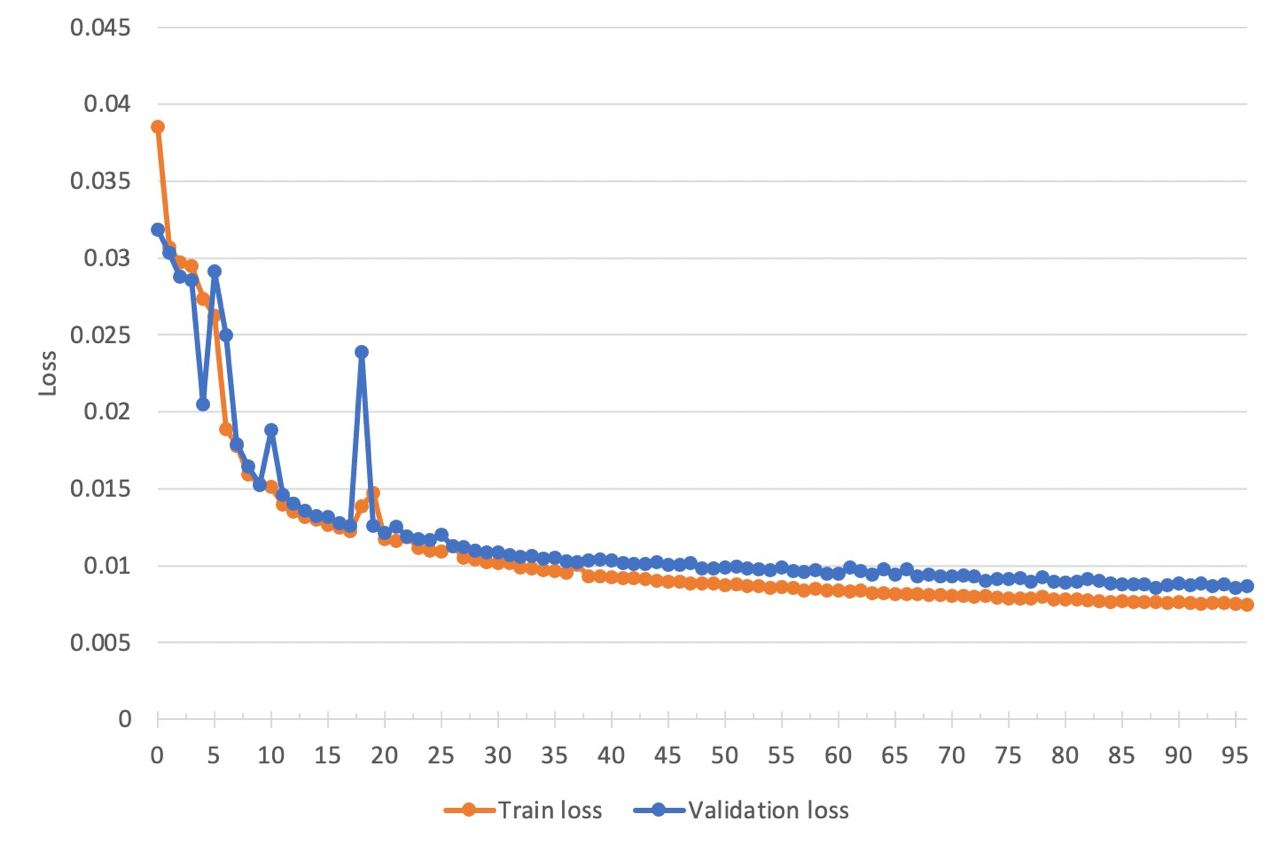
\includegraphics[width=0.5\linewidth]{bilder/nuclei/pca-2-datasets.jpg}
%		\caption{PCC with correct weight initialization converges but unstable}\label{fig:pcc-2-dataset}
%	\end{center}
%\end{figure}

As the nuclei dataset is one of the biggest ones (see Table \ref{table:data}), the experiments would first be performed on the subset of the data, and only once the training pipeline and good results were established, the training would be done using the full dataset. Figure \ref{fig:wi} (right) represents the training of nuclei using only two 96-well plates with MSE loss. The training is very unstable in the begining, but one can clearly see that the model successfully converges afterwards. Our hypothesis behind the instability was the clear lack of training data, which was proven by further training using the full data and as a result achieving a more stable PCC loss (see Figure \ref{fig:full-dataset-pcc}).

\begin{figure}[H]
	\begin{center}
		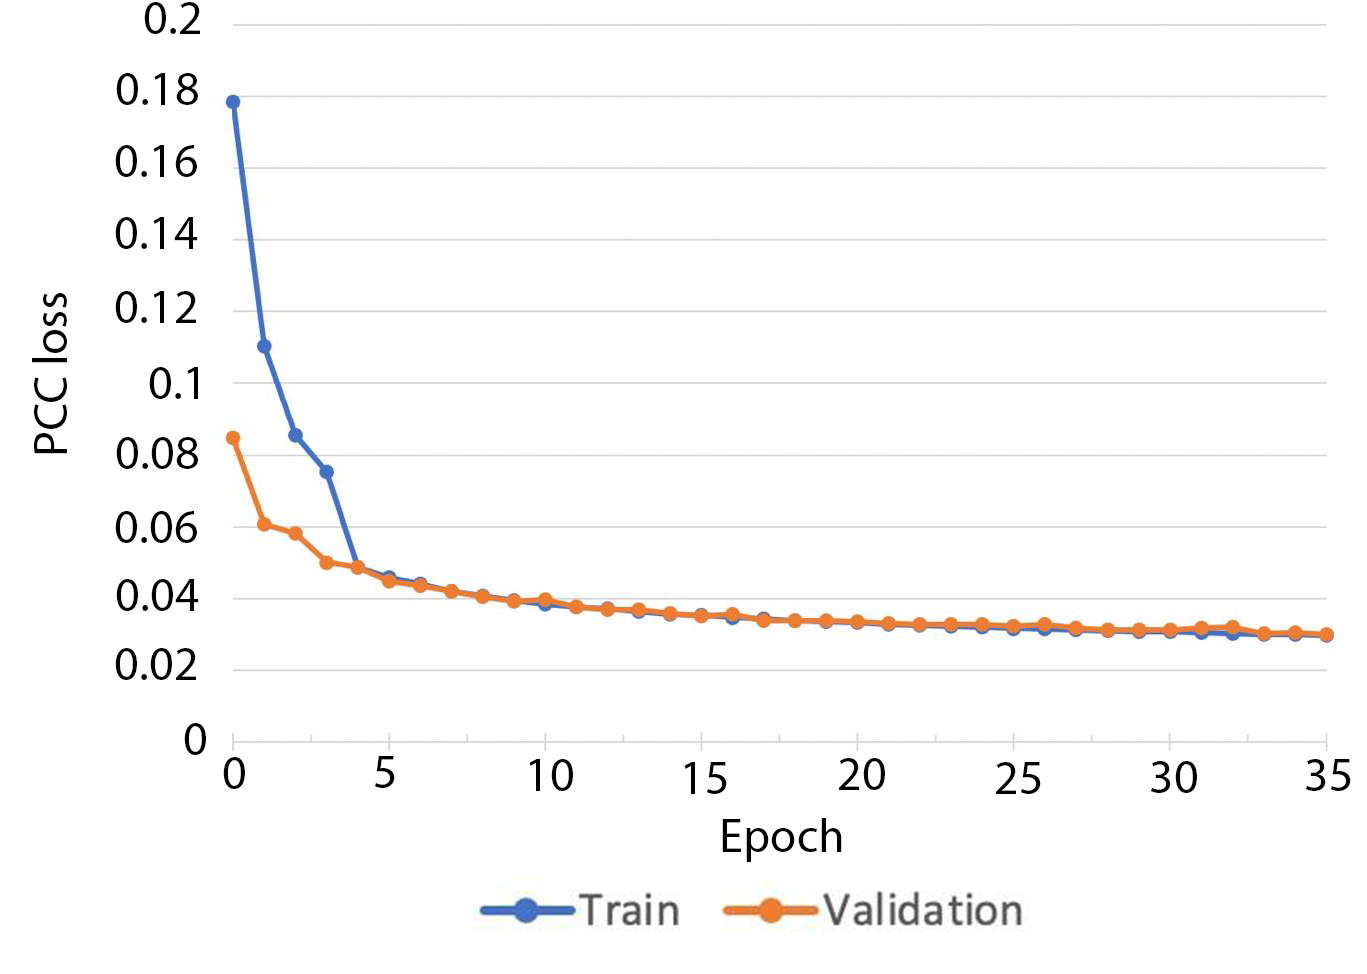
\includegraphics[width=0.5\linewidth]{bilder/nuclei/full-dataset.png}
		\caption{Having more data makes training more stable}\label{fig:full-dataset-pcc}
	\end{center}
\end{figure}

As mentioned in definition \ref{def:pcc-loss} for correct understanding of the following plots, one should be careful with differentiating PCC loss from PCC itself. PCC loss converts PCC to be between $0$ and $1$, with $0$ being an optimal value.

Seeing that the model significantly stabilizes with the use of more data and that the prediction results become much more similar to the ground truth (see Figure \ref{fig:nuclei-comparison-predictions} \textit{small dataset} vs. \textit{full dataset}), it was decided to try the use of augmentations in order to enlarge the dataset even more. In this case the augmentations were not used in order to regularize or stabilize training (by providing more difficult, for instance, blurred samples), but to simply have more data. Training and validation PCC losses from the training with the use of augmented data are presented in Figure \ref{fig:no-reg-augmented}. The augmentations used here are horizontal and vertical flips, rotations and crops (described in detail in section \ref{section:augmentations}).
\begin{figure}[H]
	\begin{center}
		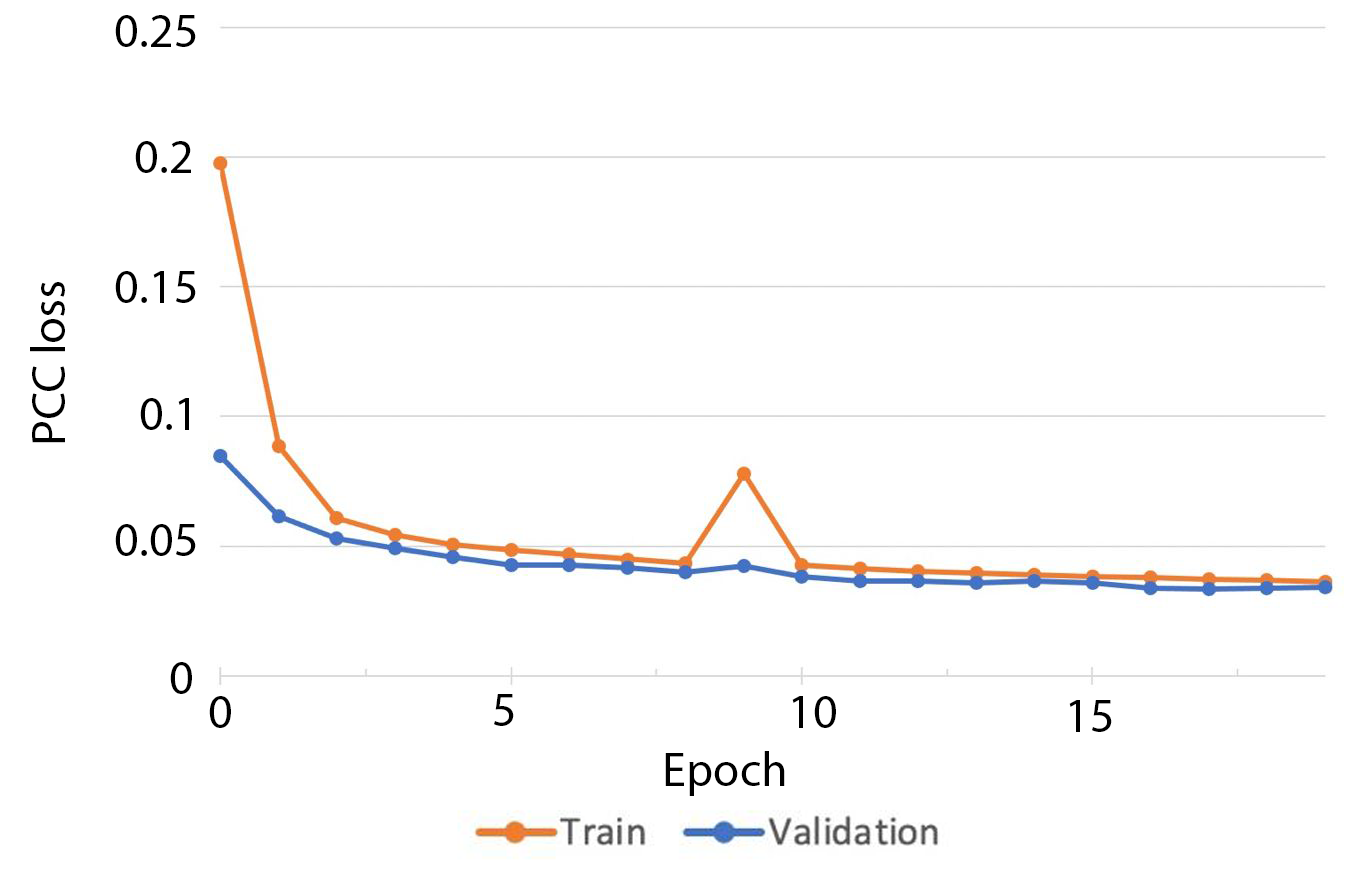
\includegraphics[width=0.5\linewidth]{bilder/nuclei/no-reg-but-aug.png}
		\caption{Adding simple augmentations in the dataset}\label{fig:no-reg-augmented}
	\end{center}
\end{figure}
Validation PCC loss has slightly increased to $0.0381$ in comparison to the previous value of $0.0365$. However, the validation set on which this loss was estimated also includes augmentations mentioned above and therefore presents a slightly more difficult task than the original validation set. True improvement is confirmed by measuring the loss of the models on the same dataset, where PCC loss has improved from $0.0365$ to $0.0322$ (or PCC from $0.92$ to $0.93$).

In the next experiment the model has additionally been regularized by adding dropout layers and using a weight decay of $0.0001$ (see Figure \ref{fig:full-dataset-pcc-regularized}). This did not bring a better result, but has only made it more difficult for the model to capture the needed feature to reproduce the fine details within the nuclei. However, this brought up a new hypothesis, namely that the model might simply have not enough of capacity to capture enough of the details. In order to confirm this a bigger model has to be trained.
\begin{figure}[htb]
	\begin{center}
		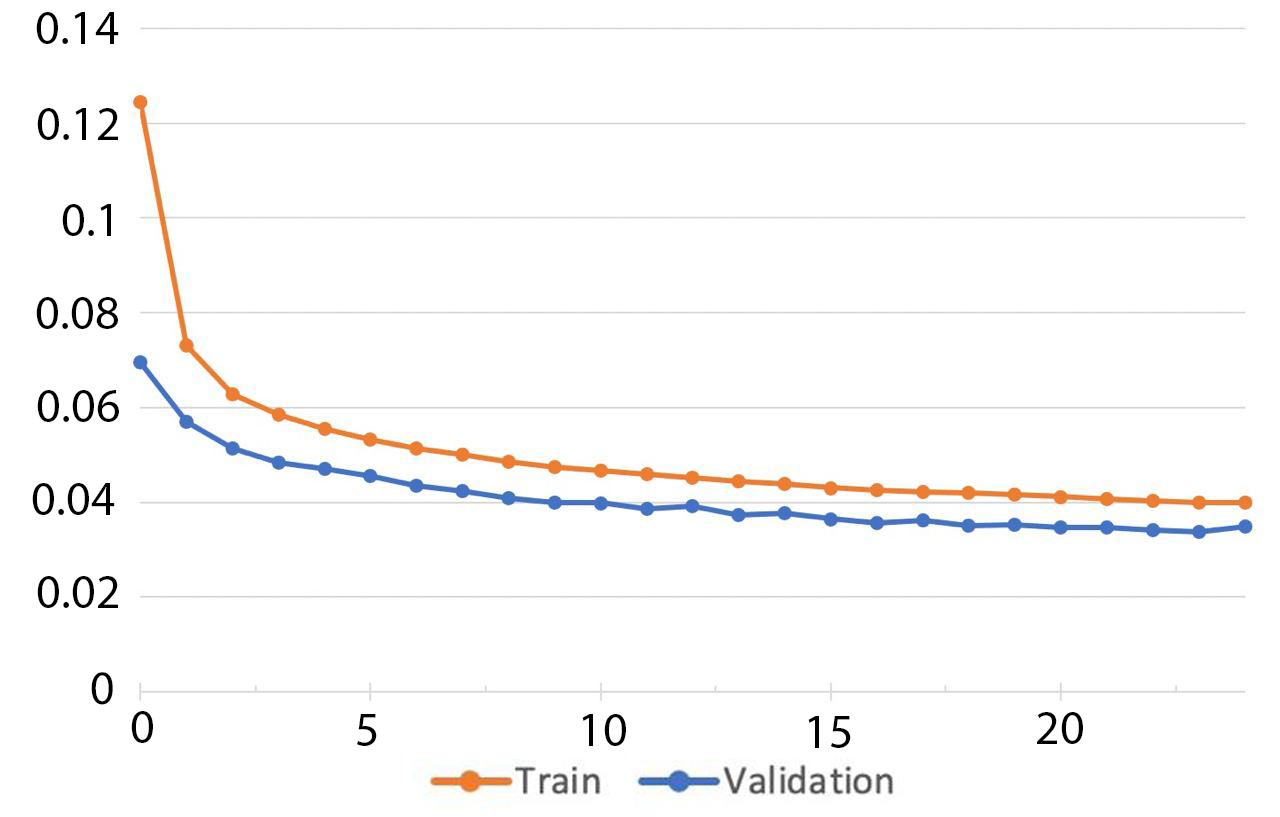
\includegraphics[width=0.5\linewidth]{bilder/nuclei/full-dataset-regularized.png}
		\caption{With regularization and augmentations}\label{fig:full-dataset-pcc-regularized}
	\end{center}
\end{figure}

\begin{figure}[htb]
	\begin{center}
		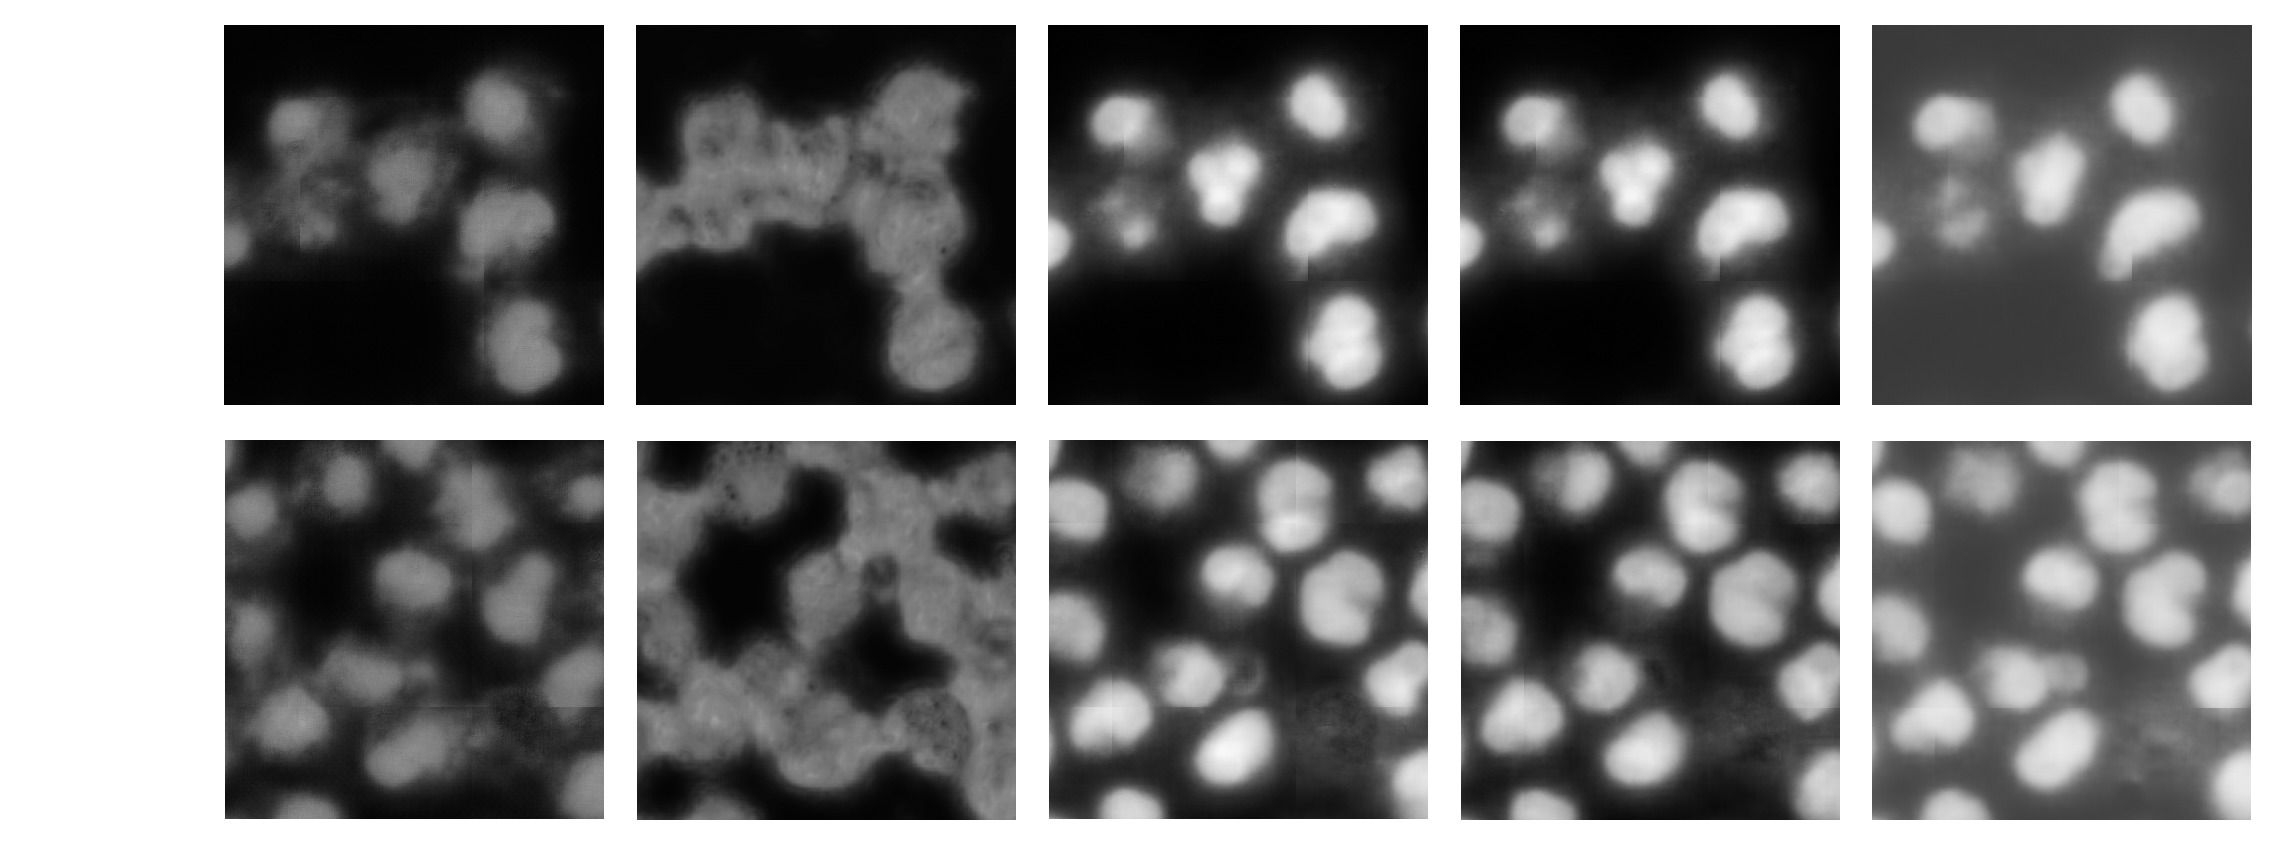
\includegraphics[width=0.6\linewidth]{bilder/nuclei/comparison-chzn-phx.png}
		\caption{Difefrent models predictions and scores comparison}\label{fig:nuclei-comparison-predictions}
	\end{center}
\end{figure}

Interestigly observations made in this section made it clear that metrics used for training (PCC and MSE losses) are indeed not representative enough to derive any conclusions regarding the model quality from them. Just by looking at Figure \ref{fig:nuclei-comparison-predictions} one can see that for example, training on the full dataset of data gives much better results than training on the small dataset. Yet MSE seems to be bigger for this experiment. Also, it is not representative in comparison of a model without the correct weight initialization vs. the regularized model with augmentations. MSE loss is much higher there, because in general the image became somewhat brighter, even though the quality of the nuclei is significantly better. PCC loss seems to represent the desired quality of the model better. This trend has been noticed by \cite{Lachance_2020} as well. They state that values of PCC lack the practical context --- which value would be good enough and good enough in which context? This issue has been addressed here as well in section \ref{section:model-evaluation}, where more practical metrics are introduced and the model evaluation on them is carried out.
